\documentclass[12pt, a4paper]{article}
\usepackage[utf8]{inputenc}
\usepackage[export]{adjustbox}
\usepackage{amsmath}
\usepackage{amsfonts}
\usepackage{amssymb}
\usepackage{xcolor}
\usepackage{graphicx}
\usepackage{subcaption}
\usepackage[left=2cm,right=2cm,top=2cm,bottom=2cm]{geometry}

\makeatletter
\renewcommand\thesubsection{\@arabic\c@subsection}
\makeatother

\newcommand{\figref}[1]{Figure~\ref{#1}}

\author{Maksym Polovyi}
\begin{document}

\begin{figure*}[t]
\centering
	\includegraphics[width=0.9\textwidth]{Images/fullSystemPicture}
	\captionsetup{justification=centering, width=0.9\textwidth}
	\caption{Snapshot of system for density $\rho = 0.95$ and $k_BT = 1.5$. Arrows represent the dipole moment of the particle. System sample obtained by means of Langevin dynamics simulation. The simulation has run for $t = 100$, with fluid medium viscosity $\eta = 1$ and particle mass $m = 1$.}
	\label{fig:fullSystemPicture}
\end{figure*}

The phenomena under study is the existence of non-zero nematic order in a colloidal suspension consisting of short-rage interacting particles. As the model, we consider colloidal particles with a permanent dipole moment $\mu \hat{m}$, where $\hat{m}$ is a unitary vector with the direction of the dipole moment. While considering a three-dimensional system, we constrain particle translational motion to a one-dimensional line, i.e. particles are confined to the $z$ axis. However, particles can explore the full three dimensional orientation space. Example of possible system configuration after running a Langevin dynamics simulation is given at \figref{fig:fullSystemPicture}.

By constraining particles to a 1D tube we effectively enforce the direction of vector $\vec{r}_{ij}$ connecting particle centers to be co-aligned with $z$ axis. Assuming that all particles have the same dipole moment $\mu_i = \mu_j = \mu$, and defining $\mu = 1$ the energy of dipole-dipole interaction for any pair (i, j) of particles is given by:
\begin{equation}
\label{eq:dipole_dipole_1D}
E_{ij}^{dip} = - \frac{1}{\Delta z^3} [3 \cos \theta_i \cos \theta_j - (\hat{m}_i \cdot \hat{m}_j)]
\end{equation}
where $\theta_i$ and $\theta_j$ are the angles between $z$ axis and dipole moments of the first and second particle respectively, and $\Delta z = |z_j - z_i|$, where $z_i$ and $z_j$ are particle positions along $z$ axis.

The repulsive part of particle-particle interaction is described by Yukawa potential
\begin{equation}
\label{eq:yukawa_interaction}
E_{ij}^{rep} = \frac{A \exp(-k \Delta z)}{\Delta z}
\end{equation}
where $A$ and $k^{-1}$ --- are the strength and range of interaction.

In this study we concentrated on the values of $A = 1000$ and $k = 10$.
Additionally, we restrict interaction to the immediate neighbors, and implement periodic boundary conditions.

We measured the following quantities:

Nematic order parameter $S$ is defined as:
\begin{equation}
\label{eq:nematic_order_parameter}
	S = \frac{3 \langle\cos^2 \theta_i\rangle - 1}{2}
\end{equation}
where $\theta_i$ it the angle between particle dipole moment and spatial axis, while angle brackets denote ensemble average.

We define particle $i$ to have Right orientation if angle $\theta_i$ is less than cut-off angle $\alpha = \pi/4$, Left orientation if $\theta_i > \pi - \alpha$, and Undefined orientation if $\alpha < \theta_i < \pi - \alpha$. 
Using this definitions, we measure the probability $P_{ij}$ of particles $i$ and $j = i+1$ have orientations respectively Right-Right, Left-Left, Right-Left and so on.

For the study of time evolution of the system, we measure the auto-correlation function for the orientation of a particle, defined as:
\begin{equation}
\label{eq:auto_corr_function}
 \Phi(t) = \langle\Phi_i(t)\rangle = \langle\cos (\theta_i(0)) \cos (\theta_i(t))\rangle
\end{equation}
where angle brackets denote ensemble average, and $t$ is simulation time.

The time evolution of the system was studied by means of Langevin dynamics (LD) simulations, using the Velocity-Verlet integration scheme, while the equilibrium results were obtained by means of Monte-Carlo (MC) simulations, and later compared with long-time LD simulations.

The MC simulations were allowed to equilibrate for $\Delta = 5 \cdot 10^5$ sweeps (one sweep consists of $N$ Monte-Carlo test steps), and after that every $\Delta$ sweeps were generated ensemble-averaged quantities, obtaining that way $10$ uncorrelated samples. LD sampling is performed directly --- each sample has different seed for random-number generator. Time-dependent results are obtained by averaging over different samples, simulated for the same LD time. The results for comparison with equilibrium results are obtained by averaging time-dependent values for times bigger than equilibration time, which is assumed to be $5 \cdot 10^3$.

As we can see on the \figref{fig:equilibrium_order_parameter}, the nematic order grows with the decrease of temperature, as well as with increase of system density. The behaviour qualitatively doesn't changes for any of the observed density and $k_BT$. Non-zero values of nematic order parameter indicates that particles tends to co- or counter-align themselves with a selected axis and therefore with each other.

\begin{figure}
 \centering
 \begin{subfigure}{.45\textwidth}
  \centering
  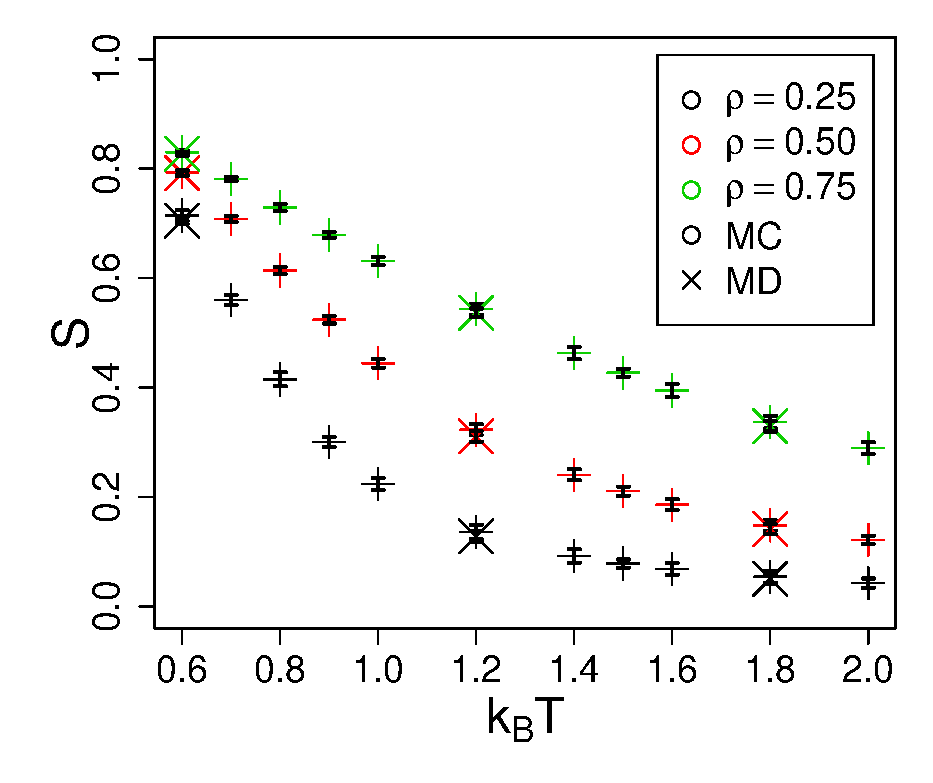
\includegraphics[width=\textwidth]{Images/op_kbt_new}
 \end{subfigure}
 \begin{subfigure}{.45\textwidth}
  \centering
  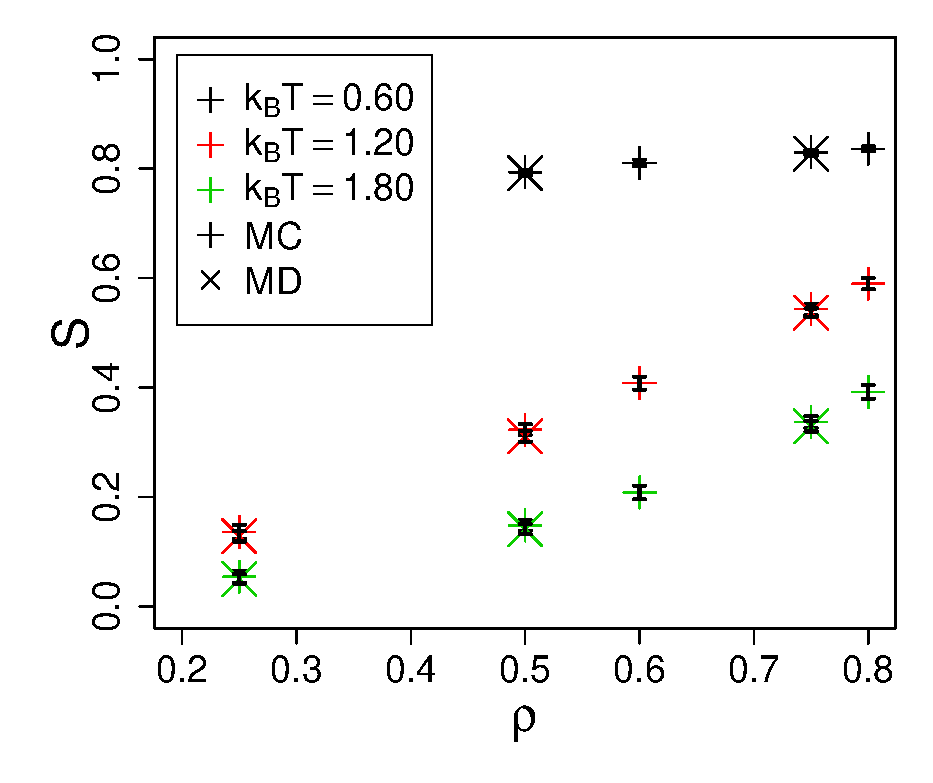
\includegraphics[width=  \textwidth]{Images/op_dens}
 \end{subfigure}
 \captionsetup{justification=centering, width=0.9\columnwidth}
 \caption{Nematic order as function of $k_BT$ for different densities(left). As function of density for different $k_BT$ (right). Vertical crosses show Monte-Carlo results averaged over $200$ samples of $3200$ particles, and diagonal crosses show Langevin dynamics results averaged over $50$ samples of $3200$ particles, and time-averaged over $t > 5 \cdot 10^3$}
 \label{fig:equilibrium_order_parameter}
\end{figure}

The particle pairs orientation probabilities (as defined above) are shown at the \figref{fig:equilibrium_orientation_prob}. As expected, the probability of two particle being co-aligned with each other is higher than to be counter-aligned. What is important to mention, however, is that probabilities of Left-Left and Right-Right configurations are the same, meaning that orientations along and against the spatial axis are indistinguishable.

The \figref{fig:dynamics_orientation_prob} shows the relaxation of particle pairs orientation probabilities for fixed density and $k_BT$. Since the simulations were run from co-aligned initial configuration, i.e. all the particles were directed along spatial axis, which corresponds to the Right orientation, the probability of Right-Right pair orientation is higher then any other. However, the relaxation taking place is exponential.

\begin{figure}
 \centering
 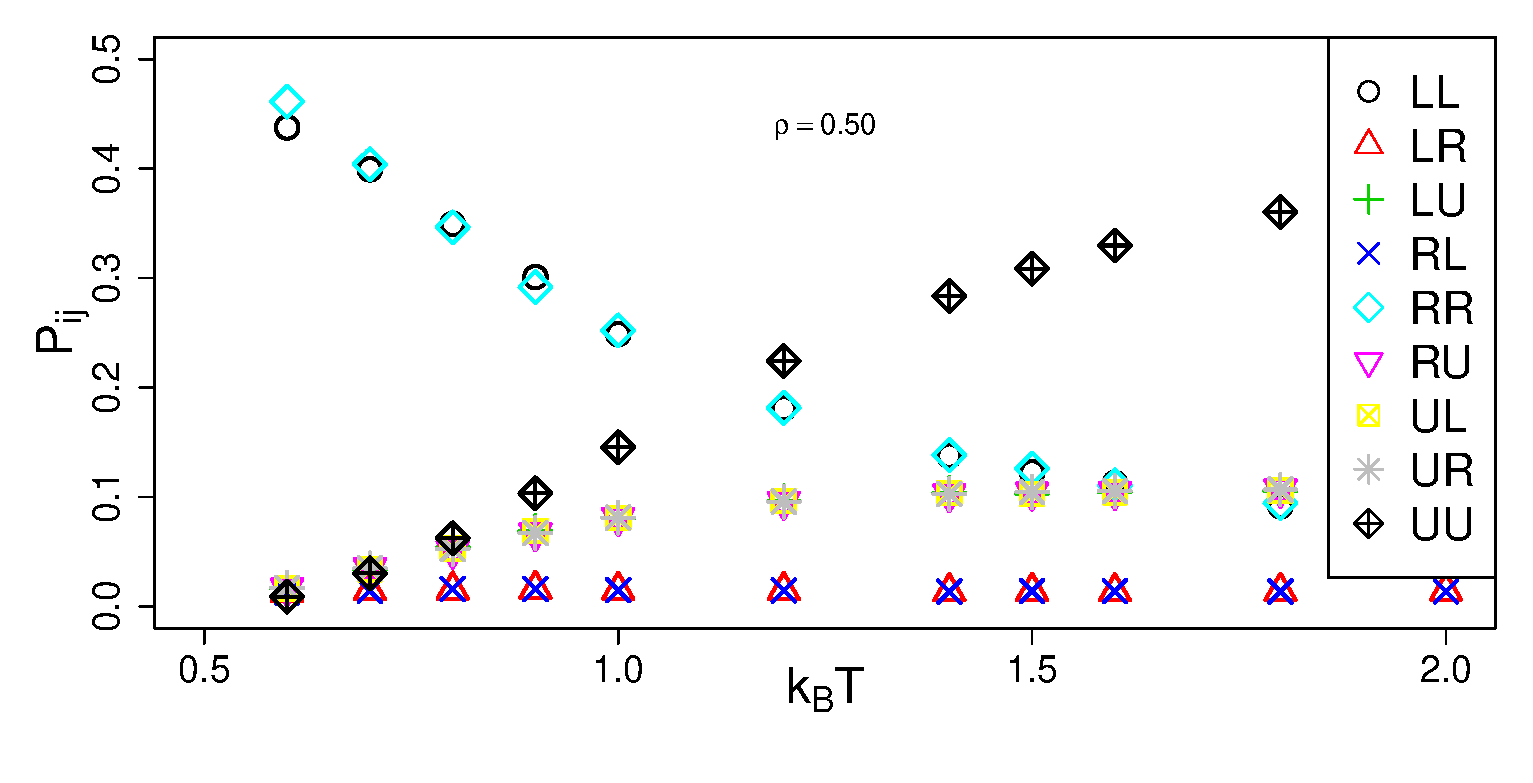
\includegraphics[width=\textwidth]{Images/particle_probs}
 \captionsetup{justification=centering, width=0.9\columnwidth}
 \caption{Equilibrium values of particle pairs orientation probabilities as function of $k_BT$ for fixed 
 $\rho = 0.5$. The results are averaged over $200$ samples of $3200$ particles.}
 \label{fig:equilibrium_orientation_prob}
\end{figure}

\begin{figure}
 \centering
  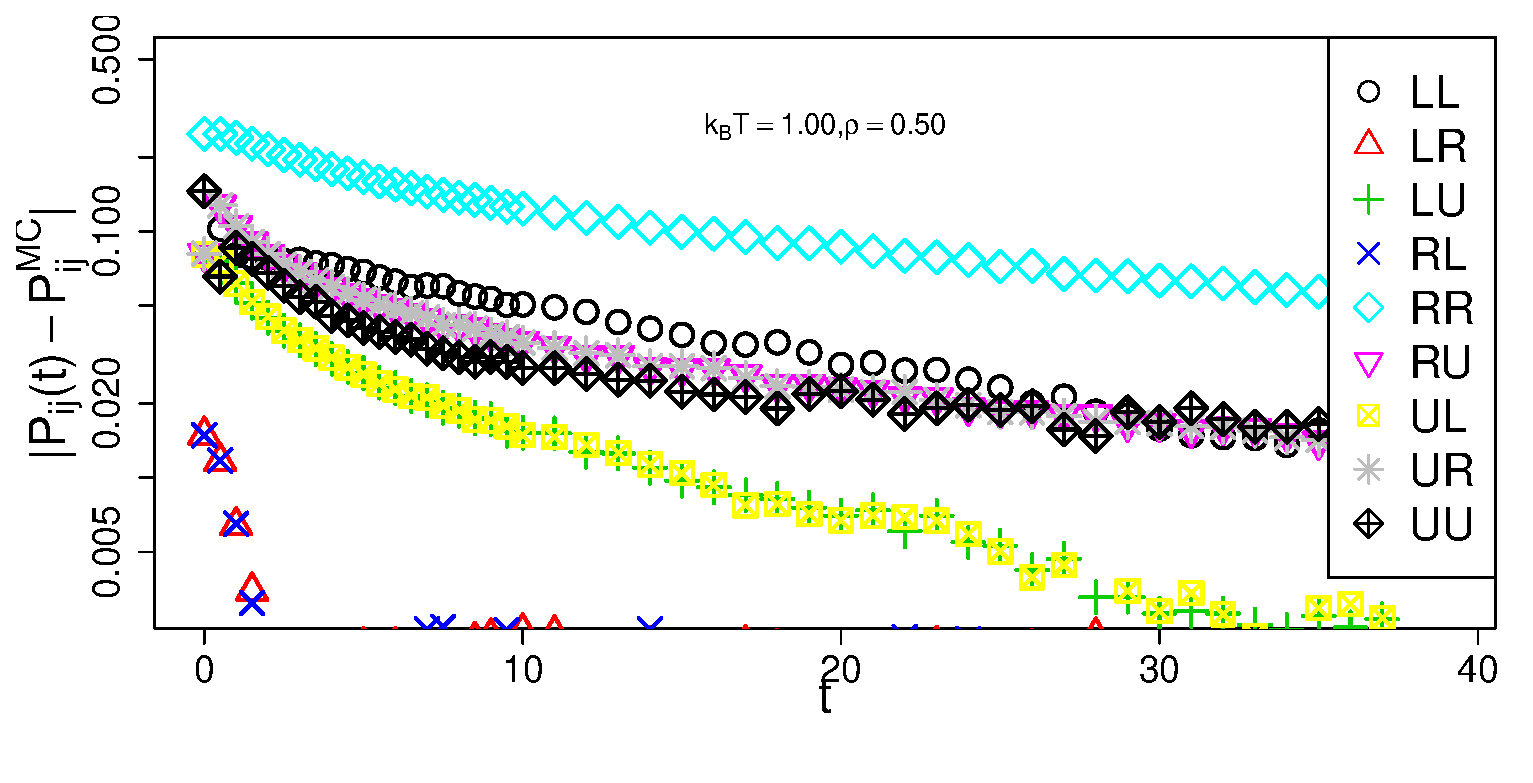
\includegraphics[width=\textwidth]{Images/particle_probs_dynamics}
 \captionsetup{justification=centering, width=0.9\columnwidth}
 \caption{Relaxation of the particle pairs orientation probabilities to the equilibrium values for fixed $\rho = 0.5$ and $k_BT = 1$. Simulation starts from completely co-aligned initial configuration. The results are averaged over $50$ samples of $3200$ particles.}
 \label{fig:dynamics_orientation_prob}
\end{figure}

As we can see on the \figref{fig:dynamics_auto_correlation_function}, in dynamical evolution particles loose information about it's initial orientation by the LD time of $40$. Prominent is the exponential decrease in auto-correlation function with time. For different initial configurations (randomly oriented over full three-dimensional space of rotations and completely co-aligned particles orientations) auto-correlation decays with the same exponent. In addition, scaling with system size is not observed.

\begin{figure}
 \centering
  \includegraphics[width=\textwidth]{Images/autocorrs}
 \captionsetup{justification=centering, width=0.9\columnwidth}
 \caption{Average auto-correlation function \eqref{eq:auto_corr_function} calculated for different system sizes with fixed $\rho = 0.75$ and $k_BT = 1.80$. Points show relaxation from completely co-aligned, and squares - from randomly-oriented initial configuration. Red values are the samples of $3200$ particles, and black are of $1600$ particles. The results are averaged over $50$ samples and binned with $\delta t = 5$.}
 \label{fig:dynamics_auto_correlation_function}
\end{figure}

\end{document}